\chapter{System Design View}

\note{
   \subsection*{Thesis = Fuzzing Hardware}
   Baiardi is interested in \textit{Fuzzing Hardware},
   he would like to do a thesis on such topic.
}

\section{System View}
\textbf{System view} is a perspective aiming to consider \textit{design rules} and consequentently \textit{vulnerabilities},
focusing on wrong design choices rather than
implementation error.
A set of design rules is used to determine the \textit{optimal} set of \textbf{controls} for a system, where \textit{optimal} indicates the smallest (i.e. \textit{cheapest} \smiley)set of controls to achieve the required robustness.\\
It is important to understand whether the optimal set of controls as imposed
by the design rules is compatible with the required performance,
and from this point of view we can define a \textbf{vulnerability} as a \textit{violation} of system design rules.

\subsection{Robustness agains Vulnerabilities}
Thus, in this scenario, designing a system means finding an acceptable \textbf{tradeoff} between \textit{design rules} and \textit{vulnerabilities}.

All the modules in an ideal system satisfy the design rules,and such ideal system is the asymptote of a sequence of distinct systems each applying more controls than the previous one as required by the design rules.\\
Any difference between the ideal system and the one being
created/under analysis may be considered as a \textbf{vulnerability},
but to decide if it is an actual vulnerability we consider the \textbf{context}
and the \textbf{cost} of the control against its usefulness.
\nl

Some differences between the ideal system and the current one cannot be avoided, supponsing some rules have been violated due to {---}possibly basic{---} performance requirements.
Other violations (i.e. \textit{missing controls}) instead may be unrelated to
performance, hence they should be fixed.\\
The key strategy to discover vulnerabilities evaluates the cost of
missing controls and compares it against
\begin{itemize}
   \item the required final \textit{performance}
   \item the \textit{risk} ($\mathcal{P}(intrusion) *impact$) due to the missing control
\end{itemize}
In a whole-system comprehensive view it is important to check \textbf{compensative controls}, i.e.
a missing control in a module may be compensated by a
control in another one.

\section{Saltzer \& Schroeder}
\labelitemize{S\&S Design Principles}{
   \begin{enumerate}
      \item \textbf{Economy of Mechanism}\\
      The protection mechanism should have a \textit{simple} and small design.
      \item \textbf{Fail-safe Defaults}\\
      The protection mechanism should \textit{deny} access by \textit{default}, and grant access
      only when explicit permission exists.
      \item \textbf{Complete Mediation}\\
      The protection mechanism should check \textit{every access} to every object.
      \note{
         Rather expensive this is the reason is one of the most hard to satisfy.
      }
      \item \textbf{Open Design}\\
      Protection mechanism should not depend on attackers being ignorant of
      its \textit{design} to successfully secure the system. 
      But may be based on the attacker's ignorance of
      specific information such as passwords or cipher keys.

      \emph{
         \color{darkgray}"An attacker who learns the key learns nothing that helps them break any message
      encrypted with a different key. That’s the essence of Kerkhoff’s principle: that
      systems should be designed that way."}
      
      \note{
         However, you should publish information on your system design \emph{iff} it results in a
         useful \textbf{peer review}.
         }
      \item \textbf{Separation of Privilege}\\
      The protection mechanism should grant access based on \textit{more than
      one piece} of information, e.g. \textit{two keys} for a safe.
      \item \textbf{Least Privilege}\\
      The protection mechanism should force every process to operate with
      the \textit{minimum privileges} needed to perform its task.
      \item \textbf{Least Common Mechanism}\\
      The protection mechanism should be shared as little as possible among users.
      \item \textbf{Psychological Acceptability}\\
      The protection mechanism should be easy to use (at least as easy as not using it).

      \note{
         Before introducing the last two principles, Saltzer and Schroeder state two things:
         \begin{itemize}
            \item Analysis of traditional physical security systems has suggested two further design principles which, unfortunately,
            apply only \textit{imperfectly} to computer systems
            \item The principles apply both to a system and to the \textit{mechanisms} we introduce to secure the system
         \end{itemize}
      }

      \item \textbf{Principle of Work Factor}\\
      Compare the cost of circumventing the mechanism against the resources of a potential attacker.
      \item \textbf{Compromise Recording}\\
      Mechanisms that reliably record a compromise of information may replace more elaborate ones that completely prevent loss.\\
      In other words,
      if you cannot be robust be aware you may be attacked and be resilient.
   \end{enumerate}
}
\subsection{Economy of mechanisms}
\begin{center}
   \textit{Keep the design as simple and small as possible}
   \note{
      \textit{KISS} rule $\longrightarrow$ \textit{\underline{K}eep \underline{I}t \underline{S}imple, \underline{S}tupid}
   }
\end{center}

"\textbf{Simple}" implies that less things can go wrong and when bugs occur, they are easier to find, understand and fix.
Vulns are proportional to the complexity of a mechanism and the code implementing it.
% = cyclomatic number to predict software bugs
When needed, complexity can be achieved by \textbf{composition} of simpler modules, and might be preferreable to building a single more comprehensive yet complex module.
\subsubsection{Designing Operating Systems}
\textbf{OS Hardening} is an approach embodying this principle:
it consists in removing useless OS functionalities for applications
of interest.\\
With respect to kernel, there are two approaches which aim to reduce complexity:
\begin{itemize}
   \item \textbf{Microkernel}\\
   Avoid the implementation of complex functions in the kernel,
   stick only to \textbf{basic} ones such as inter-process communication and basic memory management,
   possibly making room for a \textit{modular} design.
   \note{Unix and Windows do not follow this approach,
   which is instead adopted by QNX and MINIX, for instance}
   \item \textbf{Esokernel}\\
   Focus on providing \textbf{minimal abstractions} to applications and exposing as much hardware functionality as possible to applications,
   creating astrong \textbf{integration} between the OS kernel and the
   applications not only violates modularity principles
   but helps the spreading of errors.
\end{itemize}

\subsubsection{Wrapping Up}
\begin{itemize}
   \color{darkgreen}
   \item \textbf{Simplify} the interface
   \item Complex operations should be implemented by \textbf{composing}
   simple operations

\end{itemize}
\begin{itemize}
   \color{darkred}
   \item If most of the operations are rather complex (and hence
   powerful), we may be forced to enable a user to invoke a
   powerful operation just because the simple one it needs is
   missing
   \item Hence, users will apply complex operations even to
   implement simple operations and this increases their rights
   (related to the least privilege principle)
\end{itemize}

\subsection{Fail-safe and Intel \texttt{CSME}}
\begin{center}
   \textit{\ul{Base access decisions on permission rather than
   exclusion}}
\end{center}
Fail-safe related vulnerabilities are fascinating, and may be \textit{non-trivial} to abuse.
Some aspects cannot be fixed without replacing the \textit{silicon}, but only \textit{mitigated}.

Fail-safe is related to a \textit{design flaw} baked into millions of Intel chipsets:
the problem revolves around cryptographic keys that, if obtained by an attacker,
can be used to break the \textbf{root of trust} in a system.

\subsubsection{Intel Countermeasure}
Buried deep inside modern Intel chipsets there is the \textbf{Converged
Security and Manageability Engine} (\texttt{CSME}),
which is a miniature computer within a computer with its own CPU, RAM, code in a boot ROM, and with the capability to access the rest of the machine.

Currently, the \texttt{CSME}'s CPU core is 486-based, and its software is
derived from the free \textbf{microkernel} operating system \texttt{MINIX}.
\note{
   You can
   find a deep dive into the technology behind it all, sometime known
   as the Minute IA System Agent.
}
The \texttt{CSME} is digital janitor, working behind the scenes, below
operating system, hypervisor, and firmware, performing lots of
crucial low-level tasks.
\begin{itemize}
   \item Bringing up the computer, controlling power levels
   \item Starting the main processor chips
   \item Verifying and booting motherboard firmware, and providing
   cryptographic functions.
   \item The engine is the first thing to run when a machine is switched on.
\end{itemize}

\paragraph{Possible Flaw}
One of the first things the \texttt{CSME} protects is its \textbf{own built-in RAM} so that other hardware and software module cannot interfere.
However, these protections are disabled by default, there is a tiny timing gap between a system turning on and the \texttt{CSME} executing the code
in its boot ROM that installs such protections in the form of input-
output memory-management unit page tables.
During that timing gap, other hardware - physically attached or
present on the motherboard can fire off a DMA transfer into the
\texttt{CSME}’s private RAM to overwrite variables and pointers and hijack
its execution. 
At that point, the \texttt{CSME} can be controlled for
malicious purposes, all out of view of the software running above it.

Clearly this a strong \textbf{race condition}, but still possible.

\subsection{Complete Mediation}
\begin{center}
   \textit{\ul{Every access to every object must be checked for authority}}
\end{center}

This is the most crucial principle when considering performance,
since verbatim applying it would be very impactful on the system's performance.

Usually access to object is done only once on the first time,
but this leads to possible unauthorized accesses if permissions change later on.\\
Performance enhancements are achieved by caching results of
authority checks,
but they should be examined skeptically,
to avoid the above mentioned unpleasant situation.
Every uncontrolled operation that is a potential vulnerability as it may be invoked without proper rights.

\subsubsection{Fail-safe integration}
If \textbf{both} \textit{fail-safe} and \textit{complete mediation} principles are \textbf{satisfied} the system starts in a secure state and,
provided that the security kernel is correct, further on only secure transictions are enabled.
In other words, it is possible to prove security correctness using an induction approach to determine reachable states.\\
\textit{Fail-safe} plays a key role since it makes valid the base case for the induction, it acts as a "starting point".
If fail-safe default does not hold then no induction is possible
there is no base case for the induction.

\subsection{Open Design}
\begin{center}
   
   \textit{The design should \textbf{not} be secret}\\
   or\\
   \textit{Security should \textbf{not} depend on the secrecy of
   the design or of the implementation}
\end{center}
Popularly \ul{misunderstood} as
\textit{"source code should be public"} or \textit{"open-source is safer than proprietary"}.

A system \textbf{peer review} is fundamental to discover vulns in
design or implementation.
A \textit{peer review} is review made by \textbf{competent experts} which can discover flaws and vulnerabilities in a system.
So, an open source implementation is useful only if it results in a peer review, and if any peer that discovers a vulnerability communicates it
to the owner.
Instead it is useless and possibly dangerous if there are no peers available to review the code,
or they do not reveal to the owner the discovered vulnerabilities.

\begin{figure}[htbp]
   \centering
   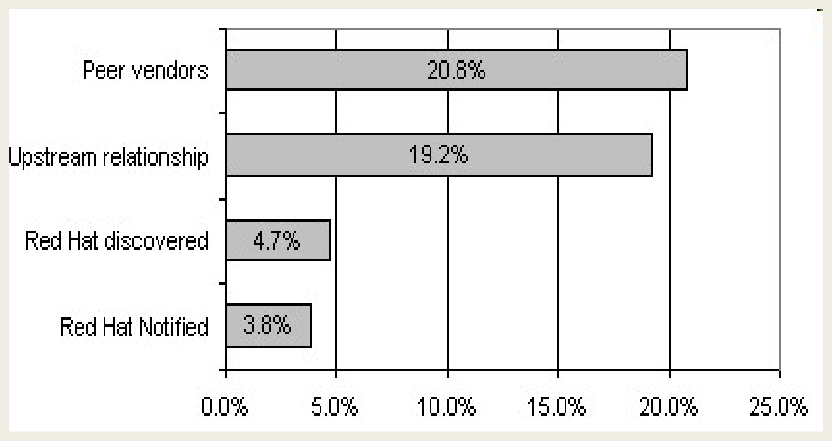
\includegraphics[width=0.45\columnwidth]{images/opendesign_redhat.png}
   \caption{RedHat vulnerabilities}
   \label{fig:opendesign_redhat}
\end{figure}
As an example, consider RedHat's statistics:
as you can see in Fig \ref{fig:opendesign_redhat}, most of the known vulnerabilities were discovered by peers,
not by RedHat's own experts.

\subsection{Separation of Privilege}
\begin{center}
   \textit{Where feasible, a protection mechanism that requires
   two keys to unlock is more \textbf{robust} and \textbf{flexible} than one
   that allows access using a single key}\\
   or\\
   \textit{Require multiple conditions to grant privilege}
\end{center}

\subsubsection{Decomposing}
A complex operation should be decomposed into simpler
operations, 
each enabled by a proper access rights,
both the complex and the simple ones.\\
In this way we can check that the subject owns both
\begin{enumerate}
   \item The right of invoking the complex $op$ (if it still exists)
   \item The right of invoking each simple $op$
\end{enumerate}

\subsection{Least Privilege}

Every subject should operate using the least set of privileges
necessary to complete its job
or
A subject should be given only those privileges it needs to complete
its task and only for the time to complete it.
\note{According to prof. Baiardi, this is the most crucial principle to be kept in mind.
Many intrusion have succeed due to the violation of this principle.}

\labelitemize{\textit{Key Points}}{
   \begin{itemize}
      \item Owning a useless access right is a \textit{vulnerability}
      \item Rights \textit{granted as needed}, \textit{revoked} after being used
      \item The \texttt{AC} matrix is a \textit{highly dynamic} data structure
      \item Rights are \textit{assigned} and \textit{revoked} as the \textit{computation evolves}
      \note{
         \footnotesize
         \item Implicitly,  \textit{Defence-in-depth}; see Fig. \ref{fig:leastprivilege_networkseg}}
   \end{itemize}
}

This principle should be applied even if the security policy is
\textbf{static},
since it defines mostly how rights should be managed \textit{after} being
granted to each subject rather than how they are granted.\\
If, in a given time interval, a subject \textit{does not need} a right
then this right should be revoked and then granted again later on by
updating the \texttt{ACM} to prevent the subject from exploiting the right in such time interval.\\
The right is removed at the beginning and then granted at the
end of the \textit{"not-needing" interval}.

\subsubsection{Protection Domain Switching}
\textbf{Protection Domain Switching} (\texttt{PDS}) consists in updating an \texttt{ACM} row,
making the same subject executed
with \textit{updated rights} in \texttt{ACM}.\\
Note that it is possible to have a \texttt{PDS} without a \textit{context switch}.
The performance overhead introduced by \texttt{PDS} is a function of the
implementation level and the adopted implementation of the
\texttt{ACM} (\textit{Capabilities} vs \texttt{ACL});
When the implementation relies on capabilities revoking a right is not trivial,
delegation and race conditions are involved.

\subsubsection{Small Domain Principle}
An alternative definition of this principle is \textbf{the small
domains principle}, to stress the importance of minimizing the
protection domains $\longrightarrow$ the number of the subject rights $\longrightarrow$ the
\textit{frequency} of the \textit{commutation} of the protection domain.\\
Besides, as the size of the protection domain decreases, it also
decreases the risk of an attack against the considered
subject.\\
If the protection domains are \textit{not small}, then we revoke access
rights when not needed and grant them again when needed, as described before.

\nl
Notice the strong relation between the two last principles
because \ul{segmented networks} force the reduction of protection
domain and separation of duties enables the implementation of
the least privilege.

\subsubsection{Common implementation}
In the classical solution a \textit{domain switching} occurs when
\begin{enumerate}
   \item A procedure (method) is \textbf{invoked}
   \item A procedure (method) \textbf{returns}
\end{enumerate}

Instead of updating row, creation (\textit{invoke}) and deletion (\textit{return}) are typically preferred.\\
When a procedure is invoked, a new row that defines its
rights is created and gets deleted when the procedure returns.
Rights are paired with the \textbf{instance} of a procedure executed
by (or on behalf of) a subject rather than with the actual procedure
code or with the subject.

The rights in the new row are a function of:
\begin{itemize}
   \item Method private variables
   \item Input parameters
\end{itemize}
The program structure in terms of \textit{classes/methods} defines the
strategy to manage rights granted to the subjects on
program data structures,
allowing automated handling of \texttt{PDS} and 
the programmer to choose the size of each protection
domain.

\subsubsection{Network Programming}
In network programming the least privilege principle is
managed through dynamic communication channels.\\
A server can be designed by introducing a distinct communication
channel for each operation implemented by the server; 
a process is \textbf{connected}\footnote{i.e. can send messages} to the channel
paired with an operation \texttt{Op} {---}{with a service \texttt{S}}{---} when it can
invoke the operation {---}{can access the service}{---};
then process is \textbf{disconnected} from the channel when it can no
longer invoke the operation.

The adoption of dynamic channels \textit{reduces} the \textbf{overhead} to reject a request by implementing in the OS kernel a mechanism to open and close ports.\\
The overhead \textit{on the server} can be further reduced by \textit{"spreding the news"}
that a message from a given node to a given port of a receiver
can be \textit{dropped} by routers or firewall;
However, this implies a larger overhead on other nodes to update \textit{routing tables} or \textit{firewall rules}.\\
On the other side, if only the final node or, even worse, the final
server can drop messages we offer an opportunity for a
\textbf{DDoS attacks} where a server is overflown by a large number of
requests to be discarded.

\subsubsection{Defence-in-depth and Network Segmentation}
\begin{figure}[htbp]
   \centering
   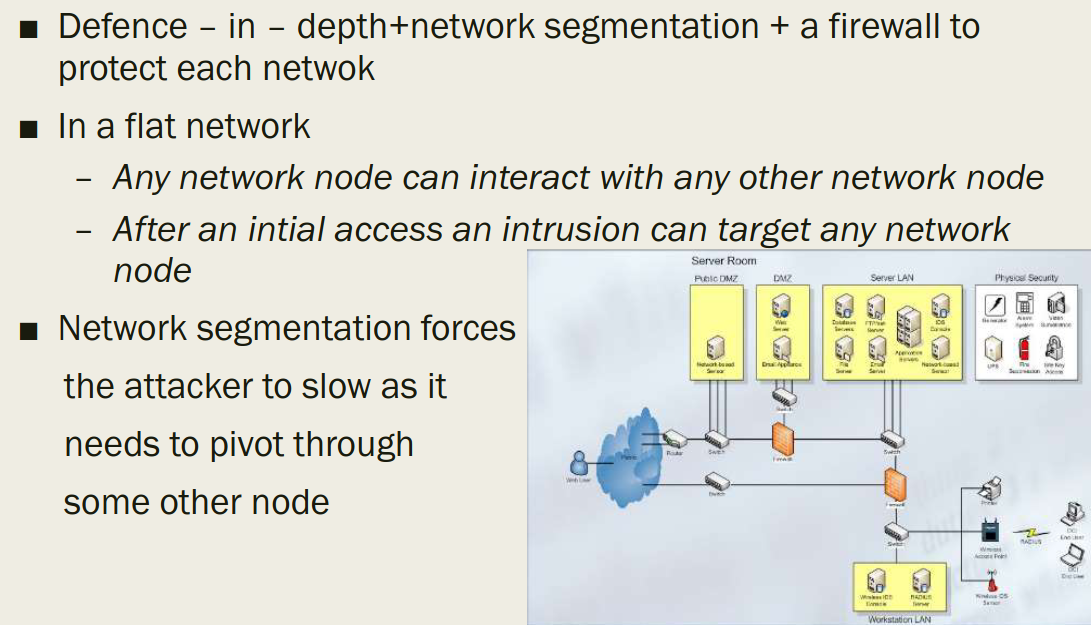
\includegraphics{images/leastprivilege_networkseg.png}\\
   \textbf{Network Segmentation} can be seen as an implementation of \textit{Defence-in-Depth} (Least Privilege key point) when designing system networks.
   \caption{Least Privilege and Network Segmentation}
   \label{fig:leastprivilege_networkseg}
\end{figure}

\subsubsection{ZeroTrust Network}

Recall that the basic idea of \texttt{ZT} is to authenticate both the \textbf{user} and the \textbf{device} exploited by the user to access a \textbf{service};
\note{
   Authenticating a device means searching for the device security status in an inventory to check the vulnerabilities that affect the device and which patches have been applied
}

\begin{figure}[htbp]
   \centering
   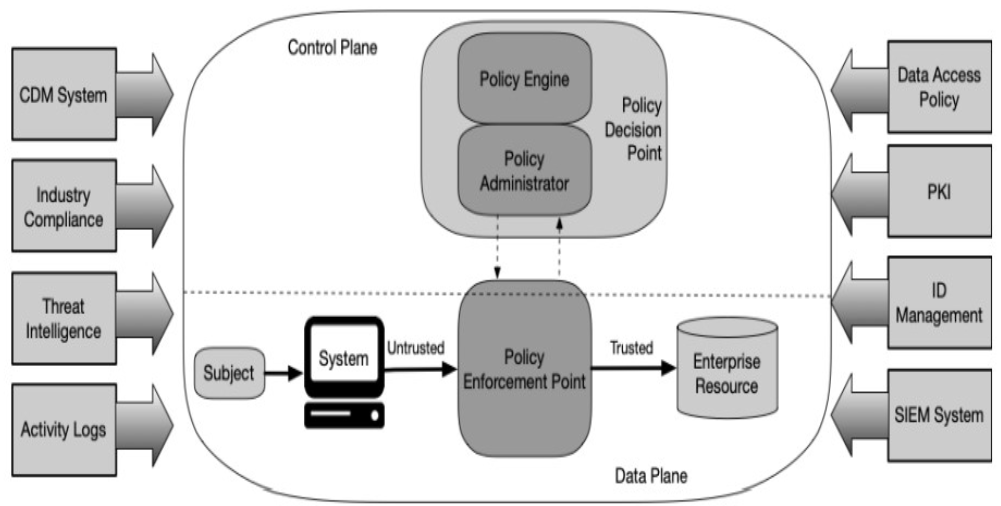
\includegraphics{images/leastprivilege_zerotrust.png}
   \caption{ZeroTrust in Networks to apply \textit{Least Privilege} principle}
   \label{fig:leastprivilege_zerotrust}
\end{figure}

\begin{enumerate}
   \item \textbf{No implicit trust} is granted to assets or user accounts based
   \textit{solely} on their physical or network location (i.e., local area networks versus the internet) or based on asset ownership
   (enterprise or personally owned).
   \item Authentication and authorization (both subject and device) are
   performed \textbf{before} establishing a session to enterprise resources
   \item Zero trust is a response to enterprise network trends that include remote users, "bring your own device" and cloud-based assets
   not located within an enterprise-owned network boundary.
   \item Zero trust protects \textbf{resources} (assets, services, accounts, etc.), \textbf{\textit{not} network segments},
   since the network location in most nowdays infrastructures is no longer the
   prime component to the security posture of the resource.

   \item All data sources and computing services are considered resources
   \item All communication is secured regardless of network location because
   location alone does not imply trust.
   \item Access to individual enterprise resources is granted on a per-session
   basis (no caching). Trust in the requester is evaluated before granting
   access with the least privileges to complete the task.
   \item Access to resources is determined by dynamic policy (= the
   observable client identity, application/ service, and the requesting
   asset) and may include behavioral and environmental attributes.
   \item The enterprise monitors and measures the integrity and security
   posture of all owned and associated assets. No asset is inherently
   trusted.
\end{enumerate}


\begin{center}
   \textit{"You cannot satisfy \textbf{ZeroTrust} unless you satisfy, at least to some degree, the \textbf{Least Privilege} principle."}
\end{center}

\subsection{Least Common Mechanism}
\begin{center}
   \textit{Minimize the amount of mechanisms common to more than
   one user and depended on by all users}
\end{center}

Instead of \textbf{sharing} \textit{mechanisms} theirselves,
the implementation usually relies on making the information flow along \textit{shared channels}, 
allowing the creation of \textbf{covert channels}.\\
Sharing should be avoided since it also decreases \textbf{isolation},
and is difficult to manage when handling Virtual machines
and Host/Network Segmentation.

Usually shared mechanisms are rather \textbf{powerful}, hence they should be \textbf{decomposed} into
simpler ones to
better satisfy the separation of privilege and least
privilege principles,
since simpler operations allow to assign to each subject \textit{only} the rights it \textit{needs}, and it is entitled to.

\subsubsection{Covert Channels}

\textbf{Covert Channels} are a means of communication between two processes that do not explicitly provide interaction mechanisms.
One process is a \textit{Trojan}, which transmits data covertly
and the other a \textit{Spy} which receives data.

\begin{enumerate}
   \item \textbf{Storage Channels}\\
   Communication is achieved by modifying a stored object.\\
   \emph{\underline{Countermeasure}} $\longrightarrow$
   shared memory areas should be always \textit{reinitialized} before being passed to another
   process,
   and they should not exist among processes with distinct security levels.
   \note{
      With cache memories information can be transmitted through faults (a page has been accessed or not)
   }
   \item Information is transmitted by affecting the relative timing of events.
   \note{
      The \texttt{Hi} \textit{Trojan} process transmits "we attack at dawn by attempting to acquire the disk drive at midnight";\\
      the \texttt{Lo} \textit{Spy} process knows that, if the disk is unavailable at midnight,
      then "we attack at dawn", otherwise, not.
   }
   Timing channels are very difficult to avoid on time-shared system but are \textbf{noisy}.
   \emph{\underline{Countermeasure}} $\longrightarrow$ Traffic Analysis and Pattern Recognition, to detect \textit{noise}.
\end{enumerate}

\subsection{Psychological Acceptability}
\begin{center}
   \textit{The human interface should be designed for ease of use so that
   users routinely and automatically accept the protection
   mechanisms correctly}\\
   or\\
   \textit{Do not adopt policies users will surely violate}
\end{center}

Security mechanisms should allow ease of installation, configuration and use,
and in general should not increase the complexity of
accessing a resource: such complexity should be hidden.

\subsection{Saltzer \& Schroeder considerations}
After defining the first 8 principles, \textit{S\&S} admit that
\begin{center}
   Analysis of traditional physical security systems have suggested
   two further design principles which, unfortunately, apply only
   \textbf{imperfectly} to computer systems
\end{center}

\begin{enumerate}
   \item Principle of \textbf{Work Factor}\\
   Compare the cost of circumventing the mechanism with the
   resources of a potential attacker
   \item Principle of \textbf{Compromise Recording}\\
   Mechanisms that reliably record a compromise of information
   may replace more elaborate ones that completely prevent loss
   \begin{enumerate}
      \item Robustness vs resilience
      \item If you cannot be robust be at least resilient
      \item At least discover successful intrusions and persistence
   \end{enumerate}
\end{enumerate}

The two principles are useful if some attacks are
successful in spite of the adoption of the previous
principles, and can be even more useful if some of such principles have been violated.
In some sense they anticipate the presence of vulnerabilities and possible failures,
reminding a system designer to not believe that they can be robust against \textit{any} adversary.

\subsection{Work Factor}
\begin{center}
   \textit{Compare the cost of circumventing the mechanism with the resources
   of a potential attacker:
   the enemy is the master and the measure}
\end{center}

The probability of a successful attack \textit{increases} with the \textbf{resources} the attacker can access,
while the cost of circumventing a mechanism is the \textbf{work factor} of the attacker.\\
So, we can consider a mechanism better than another if it can be defeated only through a larger amount of work.

The number of attacks in escalations and their attribute together with the action to collect the information on the vulnerabilities and implement the attacks determine the \textit{(minimal)} attacker work.

Measuring the amount of work the attacker (the adversary) has to do is an otput of \textbf{adversary emulation}, i.e. mimicking the attacker to understand if they can successfully attack a system.
If you have information on your adversaries then you can exploit \textit{Att\&ck Matrix} to understand if and
how they can successfully attack your system,
otherwise

\subsection{Compromise Recording}
\begin{center}
   Mechanisms that reliably record a compromise of information may replace more elaborate ones that completely prevent loss
\end{center}
A mechanism supports the discover of unauthorized use if it produces a \textbf{tamperproof record} that is reported to the owner.
It is difficult to guarantee discovery after a computer system has been attacked and controlled from the outside.
Logical damage (and internally stored records of tampering) can be undone by a clever attacker.

When collecting for security the integrity of the log is
fundamental, if the integrity of a log for security is not assured then the
log is useless.\\
The difference between a sequence of blocks and a
blockchain is a good example of the difference between
collect for debugging and collect for security

\subsection{Takeaway message}
Remember that tools do not solve security problems.
Buying a firewall doens't make a network secure, and it's not the key point.
The real problem is to understand and define the policy rules to be applied.

\section{Google System Design Strategies}

\subsection{Least Privilege}
Users should have the minimum amount of access to accomplish a task,
regardless of whether the access is performed by humans or systems.\\
Besides, since accounts may be compromised, systems should limit user access to the data and services required to do the \textbf{task at hand}.

These restrictions are most effective when you add them at the beginning of the development lifecycle,
during the design phase of new features
\note{
   security by design, as required by GDPR
}
Unnecessary privileges lead to a growing surface area for possible mistakes, bugs, or compromises, i.e. creating security and reliability risks that are expensive to contain or minimize in a running system.

In other terms:
\begin{itemize}
   \item it is better to reduce the attack surface in the \textbf{design} because this
   reduces the cost more than an update after deploying a system.
   \item the cost of security mechanisms depends upon the time when they
   are adopted, i.e. \textit{the later the more expensive}
\end{itemize}


\labelitemize{
   \textit{You should}
}{
   \begin{itemize}
      \item limit the cost of controls by prioritizing what to protect.
      Not all data or actions are created equal, and the makeup of your access may differ dramatically depending on the nature of your system.
      \item not protect all access to the same degree
      \item apply the most appropriate controls and avoid an \textit{"all-or-nothing"} mentality
   \end{itemize}
}

\labelitemize{
   \textit{You need}
}{
   \begin{itemize}
      \item to classify access based on impact, security risk, and/or criticality.
      \item to handle access to different types of data (public versus company
      versus user versus cryptographic secrets) differently
      \item to treat administrative APIs that can delete data differently than
      service-specific read APIs.
   \end{itemize}
}